\section{Mechanical design and locomotion system}
The rover central body holds the onboard computer, most of the robot's electronics, and battery.
On its front, the RGBD sensor is positioned to observe landmines in the forward direction of the rover.
Below it sit coils we use to detect metal content in the landmines in order to identify them.

In order to face the rough outdoor terrain, we designed a rocker-bogie locomotion system with six wheels.
Its main advantage is the ability to maintain contact with the ground under most circumstances.
Thus avoiding slippage and loss of maneuvrability.

The rocker-bogie is a suspension arrangement first used for the Mars Pathfinder rover by NASA.
The rocker is split in two parts
\begin{itemize}
    \item The rocker is the upper split between the front wheel and the center-rear wheels
    \item The bogie is the lower split between the center wheel and the rear wheel
\end{itemize}
The bogie is linked to the bogie with a free pivot joint allowing it to move.
The rocker is also linked to the rover body through a differential joint to balance both sides of the rover.

Each of the six wheels has a dedicated motor drive.
And each wheel is steered independently with servo motors.
Thus the rover can keep contact with the ground on very rough terrain, and maintain good maneuvrability.
This built-in redundancy also make the rover robust in case of a motor getting stuck or failing.

\begin{figure}[htbp]
   \caption{\label{fig:rover} CAD view of the rover}
   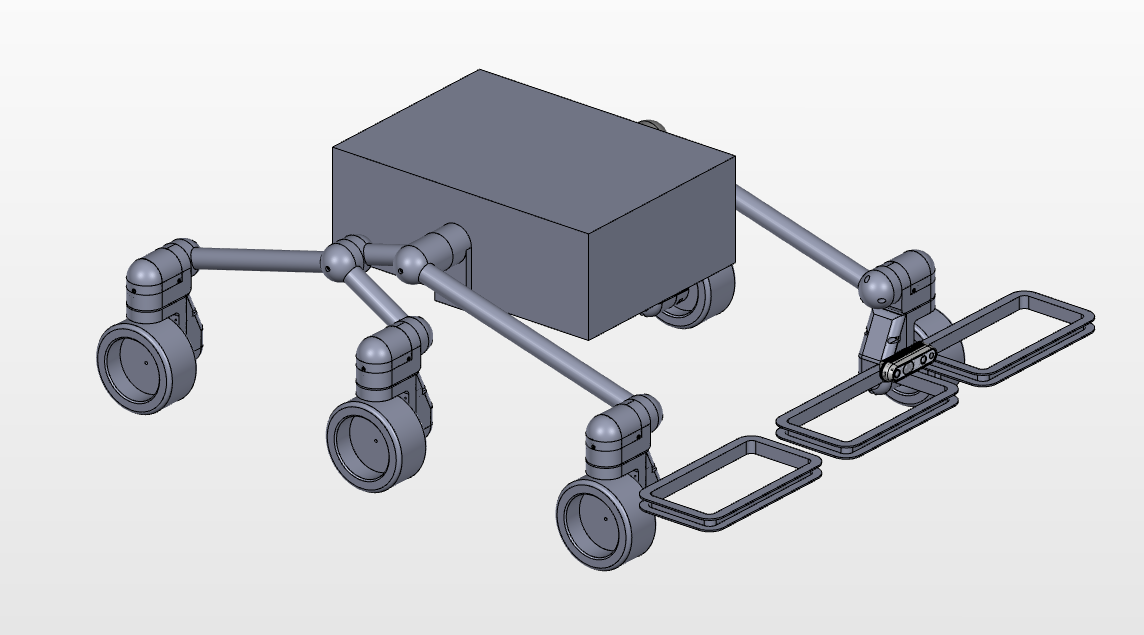
\includegraphics[width=\textwidth]{images/rover}
\end{figure}

The rocker-bogie is a 3 wheel arrangement in a tree

\section{Sensors and landmine detection}
Surface and buried mines were considered as two different detection problems and different sensors are used for either of them.

The competition rules forbid us to come in contact surface mines, so they have to be detected from as far as possible and they play a role in navigation and path planning.
The distinct shapes and colors of surface mines call for a vision based detection.
A RGBD (red-green-blue-depth) sensor was chosen to provide the imagery with which segmentation and classification algorithms will detect the landmines.

The only distinctive features of buried mines are the change in soil density that they induce and their metal content.
We decided to place an array of custom pulse induction metal detectors in front of the rover to detect the buried landmines.

\subsection{Pulse induction metal detector}
Pulse induction is a single-coil based method to detect metal at a distance.

The detector is built around a resistor-inductor circuit formed by the coil.
We charge this coil with short pulses in the range of its characteristic time-constant $\tau = \frac{L}{R}$ with $L$ the inductance and $R$ the resistance of the coil.
Then we measure the discharge signal and fit an exponential curve to it.
Three cases can arise:
\begin{itemize}
    \item Nothing is observed, hence we only observe $\tau$ of the coil
    \item Non-ferromagnetic metal is near, hence we observe a shorter $\tau$ on the discharge curve because the eddy currents generated in the metal by electromagnetic stimulation decay the magnetic field faster
    \item Ferromagnetic metal is near, hence we observe a longer $\tau$ on the discharge curve because the ferromagnetic metal will be magnetized temporarily and retains the magnetic field longer
\end{itemize}
In order to make this detection more reliable, we had to compensate for temperature drift on the measurement.
Driving the coil at high power heats it, which makes the resistance grow as $R = R_0 (1 + a T + b T^2)$ with $R_0$ the reference resistance, $a$ and $b$ characteric values of the material, and $T$ the temperature of the coil.

We built our pulse induction metal detectors using custom motor drivers, which incorporate power electronics to turn the on and off the supply current to the coil and a shunt resistor to measure the induced current.

\subsection{RGBD Sensor}
A complementary detection mechanism is implemented using an RGBD sensor.
From the sensor data we build a local point cloud of the scene in front of the rover.
Then, we segment it to extract objects from the ground.
Objects that fit the geometric and color description of a landmine are logged.


\section{Electronic circuit and control system}
The electronics of the rover are summarized by the block diagram in figure \ref{fig:block-diagram}.
The diagram is color-coded:
\begin{itemize}
    \item Power components are represented in red
    \item Wireless communication devices are represented in green
    \item CAN-bus connected devices are represented in blue
\end{itemize}

\begin{figure}[htbp]
   \caption{\label{fig:block-diagram} Block diagram of the rover electronics}
   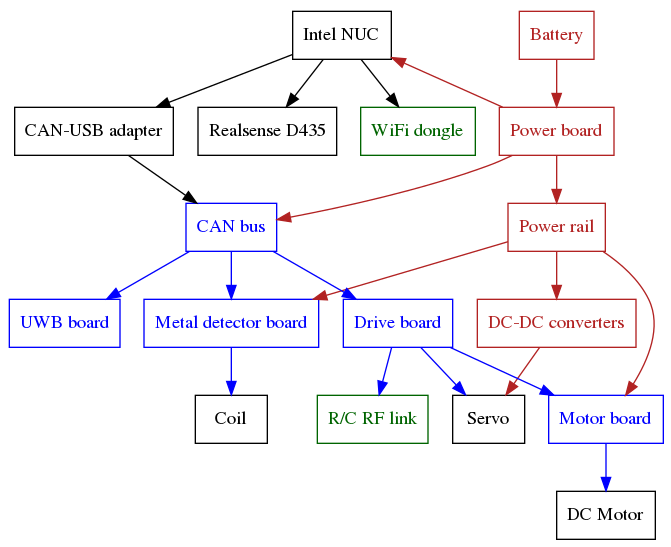
\includegraphics[width=\textwidth]{images/diagram}
\end{figure}

Each wheel has a custom motor control board to drive it, and a steering servo motor for direction.
All servo motors are driven by a custom drive board that interfaces motor control boards too.
The drive board exposes a differential control interface to the whole rover locomotion which can then be controlled either manually via the RF link with a remote control, or autonomously via the onboard computer.

An onboard computer (Intel NUC) aggregates information from all sensors to build the map of mines.
The RGBD sensor we use is an Intel Realsense D435 interfaced over USB 3.1.
The computer also connects to the CAN-bus to receive position information from our custom UWB beacon board.
It also retrieves signals from the custom metal detector board that drives the coil.

A custom power board protects all circuitry from the battery.
It allows a us to monitor battery discharge, provides some security (fuses), and DC-DC voltage conversion.
From this power board we dispatch power for the onboard computer and the CAN-bus command voltage (+5V).
Then the protected battery voltage is dispatched through a power rail to all actuators: the coils, the DC motors, and the servo motors.
Note that each servo motor is powered by a dedicated DC-DC converter to provide it with a more stable power source.


\section{Area navigation}
Our navigation is simple but open for extension.
The rover will be manually driven, however everything is such that the onboard computer could control the rover.
The idea is the cover the field in a grid pattern, while going around any landmines we encounter.

The design is such that we first aim to drive the rover manually by remote control.
This way we can cover the whole minefield with a grid path while avoiding surface mines.

Further development would allow our onboard computer to move the rover autonomously across the minefield.
The onboard computer running ROS for sensor processing and map building, would also run path planning to drive the rover around.
Path planning can be implemented with the ROS navigation stack.
By design, the ROS navigation stack\footnote{\url{http://wiki.ros.org/navigation}} allows a robot to be controlled as long as it exposes a differential drive interface.
The RGBD sensor can be used to provide pseudo laserscan measurements for obstacle avoidance, these can be configured to avoid surface mines correctly.
A grid plan covering the minefield can be decomposed into waypoints to ensure the rover covers it well enough.
This can be extended by using an exploration maximization approach such as the hector exploration planner developed by TU Darmstadt\footnote{\url{http://wiki.ros.org/hector_exploration_planner}}.

\section{Mapping}

To map the competition area, our robot will use a custom localization system that we developped.
Similarly to GPS, our system computes the rover's position by using the \gls{rtt} of a radio signal to several fixed beacons, of which the position is known.

We use Decawave's DWM1000 radio modem with a custom protocol to measure the distance.
This gives us a good distance measurement accuracy: $1 \sigma = \SI{3}{\centi\meter}$.

Since we know the distance to each fixed beacons, as well as their positions, we can compute the position of the robot.
This is done using an \gls{ekf}, using the distance to a point as a correction function.
For the prediction step, we originally planned to use an inexpensive \gls{imu}, similar to the ones found in mobile phones.
However we probably won't implement it, due to time constraints.

The system was already tested on a \SI{20}{\meter} by \SI{20}{\meter} open field at our workshop.
We got very good positioning results and reliability, although we lacked time to do a quantitative analysis of the measurement accuracy and precision.
According to simulation, we should be within \SI{10}{\centi\meter} of ground truth.
As the reliability so far is good, we will be using this system only for Minesweepers 2018.


\section{Rough environment handling}
With its rocker-bogie locomotion system, the rover is designed to be very forgiving to navigation errors in rough terrain.
In addition, the independently actuated wheels allow for tight turn radii without slippage.

In order to be able to test and validate changes in the mechanical design as quickly as possible, most of the rover's parts are manufactured using 3D printing technologies.
A future iteration of the mechanics would replace the plastic parts with metal for better robustness against harsh environments and a stiffer locomotion system.

Autonomous path planning around obstacles in rough terrain can be achieved with the on-board depth sensor.


\section{Video}
